\subsection{Skill Recovery with Balanced Self-Imitation}
Balanced self-imitation raises reaching success from 8.0\% to 31.1\% (Fig.~\ref{fig:retention}). Plate placement changes from 50.0\% to 52.3\%, and bowl placement from 23.05\% to 27.65\%. The bank combines earlier reaching successes with current placement successes. Each skill is evaluated under its own fixed reset protocol; placement skill tests can begin with a held object.

\begin{figure*}[!t]
\centering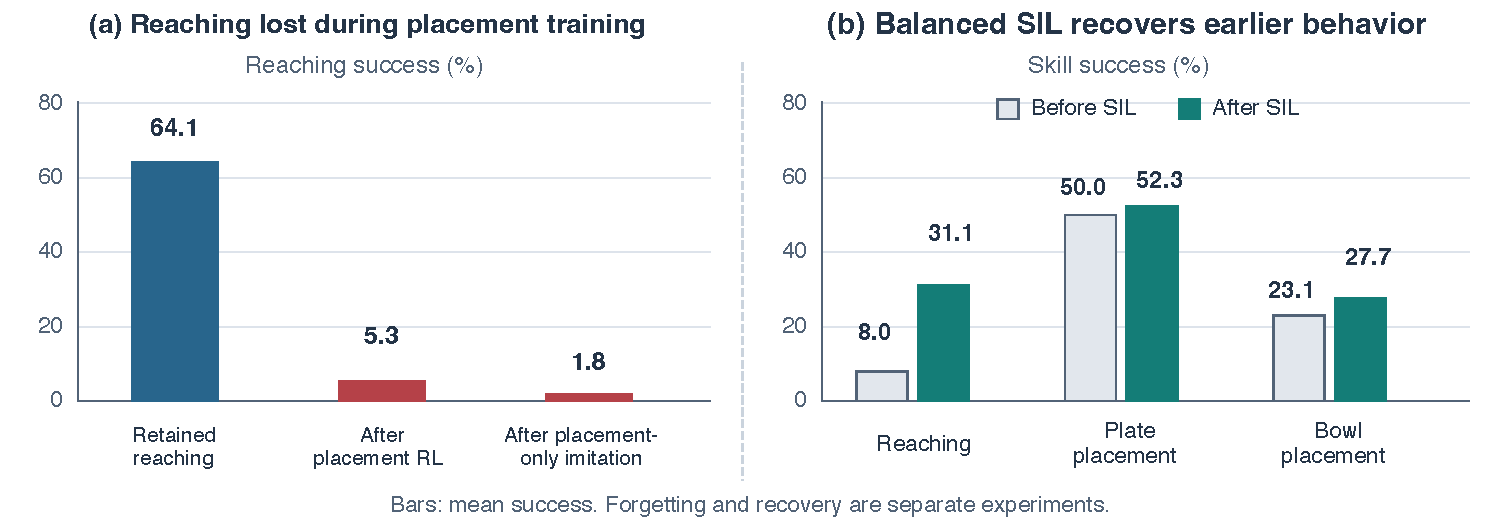
\includegraphics[width=\textwidth]{figures/skill_retention.pdf}
\caption{Skill success before and after balanced self-imitation. Bars show means across three evaluation rounds for reaching and two rounds for each placement skill, per condition. Reaching partially recovers while both placement means increase.}
\label{fig:retention}
\end{figure*}

Recovery is partial, with placement performance retained while reaching improves. These skill-level results do not isolate the contribution of self-imitation to final full-task success.
